% Created 2019-12-17 mar 15:16
% Intended LaTeX compiler: pdflatex
\documentclass[11pt]{article}
\usepackage[utf8]{inputenc}
\usepackage[T1]{fontenc}
\usepackage{graphicx}
\usepackage{grffile}
\usepackage{longtable}
\usepackage{wrapfig}
\usepackage{rotating}
\usepackage[normalem]{ulem}
\usepackage{amsmath}
\usepackage{textcomp}
\usepackage{amssymb}
\usepackage{capt-of}
\usepackage{hyperref}
\author{Víctor Chico Rodríguez}
\date{\today}
\title{Referencia JAVA}
\hypersetup{
 pdfauthor={Víctor Chico Rodríguez},
 pdftitle={Referencia JAVA},
 pdfkeywords={},
 pdfsubject={},
 pdfcreator={Emacs 26.3 (Org mode 9.1.9)}, 
 pdflang={Spanish}}
\begin{document}

\maketitle
\tableofcontents

\href{./referenciajava.org}{Descargar archivo fuente .org}\\
\href{./referenciajava.pdf}{Descargar como PDF}

\section{Introducción}
\label{sec:orge49cecd}
Java es un lenguage de programación orientado a objetos, se creó en 1996 y está basado en C++, es un lenguaje que se ejecuta en una máquina virtual que interpreta (la JVM, siglas de \emph{Java Virtual Machine}) las instrucciones compiladas a bytecode (El lenguaje de la máquina virtual)
\subsection{Estructura de un programa}
\label{sec:org6160106}

\begin{verbatim}
//Este fichero pertecene al paquete (carpeta) curso.java.manual (curso/java/manual)
package curso.java.manual;

//Esto es una importación de la clase Scanner del paquete java.io
import java.io.Scanner;

//Esto es una clase pública que se llama HolaMundo
public class HolaMundo {

    /*Este es el método main (principal), 
es un método especial que servirá comom punto de entrada a la aplicación. 
Este método es:
- público (puede ser accedido desde cualquier clase)
- estático (puede ser accedido sin necesidad de crear un objeto de la clase
-  no devuelve nada (tipo void)
- recibe como argumentos un array (matriz) de objetos de tipo String (cadena de texto)
*/
    public static void main (String [] args) {
	//Este es un objeto de la clase Scanner que se llama scan
	//Este objeto se inicializa con la palabra reservada new y
	//recibe como argumento System.in (Entrada del sistema)
	Scanner scan = new Scanner(System.in);

	/*
	  Esto es una llamada a un método, concretamente al método print(String)
	  del atributo out de la clase System, este método imprime en la pantalla
	  (consola de texto) el texto que se le pase como parámetro y continúa
	  en la misma línea.
	  Como parámetro se le pasa la cadena de texto (String) "¿Cómo te llamas?"
	  Los valores de tipo String van siempre entre comillas dobles "
	 */
	System.out.print("¿Cómo te llamas?");

	//Este es un objeto de la clase String (cadena de texto) que se llama nombre.
	//Este objeto se inicializa automáticamente con el valor que devuleve
	//el método readLine() (Método sin argumentos) del objeto scan.
	String nombre = scan.nextString();

	/*
	  Esto es otra llamada a un método, en este caso al println del atributo
	  out de la clase System, nótese la diferencia con la llamada anterior
	  (print -- println), ese ln añadido lo que hace es saltar de línea una
	  vez haya impreso lo que le pasemos como parámetro.

	  En este caso, como parámetro se le pasa una cadena de texto (igual que antes)
	  con el valor "Hola, " a lo que le concatenamos (sumamos) el valor de 
	  la variable nombre
	 */
	System.out.println("Hola, "+nombre);
    }
}
\end{verbatim}
\captionof{figure}{\label{org40d9b97}
Hola Mundo}

\section{Tipos de datos}
\label{sec:org82b8f94}
Los tipos de datos primitivos en java son los siguientes:
\begin{center}
\begin{tabular}{lll}
tipo & descripción & clase asociada\\
\hline
byte & número entero de 8 bits (-128 a 127) & Byte\\
short & número entero de 16 bits (-32768 a 32767 & Short\\
int & número entero de 32 bits (\(-2^{32}\) a \(2^{32}\)) & Integer\\
long & número entero de 64 bits (\(-2^{64}\) a \(2^{64}\)) & Long\\
float & número decimal de 32 bits & Float\\
double & número decimal de 64 bits & Double\\
boolean & valor booleano o lógico (verdadero o falso) & Boolean\\
char & caracter de texto (único) & Character\\
\end{tabular}
\end{center}


Los tipos de datos normalmente se usan en su forma primitiva (columna tipo) y se pueden asignar directamente, pero a veces es util usar métodos de su clase asociada.
\section{Operadores}
\label{sec:org3890b99}
\subsection{Asignación}
\label{sec:org4224b6a}
El operador \textbf{=} se usa para asignar valores a variables:
\begin{verbatim}
int a = 0;
\end{verbatim}
\subsection{Aritméticos}
\label{sec:org733cb3d}
En java se pueden realizar multitud de operaciones matemáticas con la misma precedencia que en la vida real, si se necesita modificar se pueden utilizar paréntesis, los operadores aritméticos son los siguientes:
\begin{center}
\begin{tabular}{ll}
Operador & Descripción\\
\hline
\textbf{+} & Operador de suma\\
\textbf{-} & Operador de resta\\
\textbf{*} & Operador de multiplicación\\
\textbf{/} & Operador de división\\
\textbf{\%} & Operador de resto de la división\\
\end{tabular}
\end{center}

El siguiente código es una pequeña demostración de los operadores mencionados:

\begin{verbatim}

public class Aritmeticos {

     public static void main (String[] args) {

	 // Variable de tipo int que tendrá como valor el resultado de 1 + 2
	 int resultado = 1 + 2;
	 // El valor de resultado es 3
	 System.out.println("1 + 2 = " + resultado);
	 int resultado_original = resultado;

	 // Los operadores se pueden usar entre variables (numéricas) y números
	 // en este caso se resta 1 al valor de resultado primero y se asigna a
	 // la variable resultado después
	 resultado = resultado - 1;
	 // El valor de resultado es 2
	 System.out.println(resultado_original + " - 1 = " + resultado);
	 resultado_original = resultado;

	 // Multiplicamos el resultado por 2 y lo volvemos a asignar a la variable
	 //resultado
	 resultado = resultado * 2;
	 // El valor de resultado es 4
	 System.out.println(resultado_original + " * 2 = " + resultado);
	 resultado_original = resultado;

	 // Dividimos el resultado entre 2 y lo asignamos
	 resultado = resultado / 2;
	 // El valor de resultado es 2
	 System.out.println(resultado_original + " / 2 = " + resultado);
	 resultado_original = resultado;

	 resultado = resultado + 8;
	 // El valor de resultado es 10
	 System.out.println(resultado_original + " + 8 = " + resultado);
	 resultado_original = resultado;

	 // Dividimos el resultado entre 7 y nos quedamos con el resto, luego lo
	 // asignamos
	 resultado = resultado % 7;
	 // El valor de resultado es 3
	 System.out.println(resultado_original + " % 7 = " + resultado);
     }
 }
\end{verbatim}
\captionof{figure}{\label{orgff3d71b}
Aritmeticos}

Como vimos anteriormente, el operador suma \textbf{+} se puede utilizar también para concatenar texto:

\begin{verbatim}
class Concatenacion {
    public static void main(String[] args){
	String firstString = "Esto es";
	String secondString = " una cadena de texto concatenada.";
	String thirdString = firstString+secondString;
	System.out.println(thirdString);
    }
}
\end{verbatim}
\captionof{figure}{\label{org1245f92}
Concatenación}


\subsubsection{Operadores unarios}
\label{sec:orgbc33015}
En java hay un tipo de operadores aritméticos que sólo se utilizan en un operando, son los operadores unarios:
\begin{center}
\begin{tabular}{ll}
Operador & Descripción\\
\hline
+ & Indica un valor positivo\\
- & Indica un valor negativo\\
++ & Incrementa en 1 el valor\\
-- & Decrementa en 1 el valor\\
! & Invierte el valor de un booleano\\
\end{tabular}
\end{center}

\begin{verbatim}
class Unarios {
    public static void main(String[] args) {
	int resultado = +1;
	// El resultado es 1
	System.out.println(resultado);

	resultado--;
	// El resultado es 0
	System.out.println(resultado);

	resultado++;
	// El resultado es 1
	System.out.println(resultado);

	resultado = -resultado;
	// El resultado es -1
	System.out.println(resultado);

	boolean exito = false;
	// false
	System.out.println(exito);
	// true
	System.out.println(!exito);
    }
}
\end{verbatim}
\captionof{figure}{\label{org96f9d58}
Unarios}

Los operadores de incremento y decremento (\textbf{++} y \textbf{--}) actuan de manera diferente dependiendo de si se ponen delante o detrás del valor a modificar, si se usan de manera prefija \texttt{++variable} el valor se incrementa primero y la variable se usa después (ya incrementada), si se usa de manera postfija \texttt{variable++} se utilizará el valor de la variable sin incrementar y luego se incrementará:

\begin{verbatim}
class PrePost {
    public static void main(String[] args){
	int i = 3;
	i++;
	// imprime 4
	System.out.println(i);
	++i;			   
	// imprime 5
	System.out.println(i);
	// imprime 6
	System.out.println(++i);
	// imprime 6
	System.out.println(i++);
	// imprime 7
	System.out.println(i);
    }
}
\end{verbatim}
\captionof{figure}{\label{org1b16681}
Prefijos y Postfijos}

\subsection{Lógicos}
\label{sec:org074f151}
Son operadores que devuelven valores lógicos (verdadero o falso)
\begin{center}
\begin{tabular}{ll}
Operador & Descripción\\
\hline
== & igual que\\
!= & distinto que\\
> & mayor que\\
>= & mayor o igual que\\
< & menor que\\
<= & menor o igual que\\
\&\& & Y lógico\\
\(\vert{} \vert{}\) & Ó lógico\\
instanceof & Objeto pertenece a clase\\
\end{tabular}
\end{center}

Normalmente estos operadores se utilizarán en sentencias que requieran un valor lógico, como los condicionales o los bucles, de los que hablaremos más adelante, en este ejemplo vemos como, en base a los valores 1 y 2, que operaciones se ejecutan y cuales no:

\begin{verbatim}
class Comparacion {

    public static void main(String[] args){
	int valor1 = 1;
	int valor2 = 2;
	System.out.println ("valor1="+valor1+", valor2="+valor2);
	if(valor1 == valor2) {
	    System.out.println("valor1 == valor2 --> " + (valor1 == valor2));
	}
	if (valor1 != valor2) {
	    System.out.println("valor1 != valor2 --> " + (valor1 != valor2));
	}
	if (valor1 > valor2) {
	    System.out.println("valor1 > valor2 --> " + (valor1 > valor2));
	}
	if (valor1 < valor2) {
	    System.out.println("valor1 < valor2 --> " + (valor1 < valor2));
	}
	if (valor1 <= valor2) {
	    System.out.println("valor1 <= valor2 --> " + (valor1 <= valor2));
	}
    }
}
\end{verbatim}
\captionof{figure}{\label{org97476bd}
Comparación}

A veces es interesante comprobar si una comprobación cumple mas de una condición o si una sentencia se ejecutará si se cumple alguna de las condiciones posibles, es en este caso que utilizaremos los operadores lógicos \texttt{\&\&} y \texttt{||}.

\begin{verbatim}
class Condicionales {

    public static void main(String[] args){
	int valor1 = 1;
	int valor2 = 2;
	if((valor1 == 1) && (valor2 == 2))
	    System.out.println("valor1 es 1 AND (Y) valor2 es 2");
	if((valor1 == 1) || (valor2 == 1))
	    System.out.println("valor1 es 1 OR (O) valor2 es 1");
    }
}
\end{verbatim}
\captionof{figure}{\label{orgd53e07c}
Operadores Condicionales}

\section{Condicionales}
\label{sec:org8921a50}
En java tenemos principalmente dos estructuras condicionales, la primera es la que se compone con las sentencias \texttt{if} y \texttt{else}, y la segunda es la sentencia \texttt{switch}.

\subsection{if y else}
\label{sec:org51e3312}
La sentencia \texttt{if} se escribe de la siguiente manera:
\begin{verbatim}
if (condicion) {
    proceso;
}
\end{verbatim}
Donde \texttt{condicion} es un valor booleano (lógico), que puede ser una variable de tipo boolean, un valor \texttt{true} o \texttt{false} directamente, aunque no tuviera mucho sentido en este caso, o el resultado de una comparación como las que acabamos de ver.

Si la condición se cumple el \texttt{proceso} (que puede ser un número indeterminado de sentencias) se ejecuta, si no se cumple, no se ejecuta, decimos que se produce un salto condicional.

Hay veces que queremos que si se cumple una condición se ejecute un determinado código y, si no se cumple, otro, esto lo conseguimos con la sentencia \texttt{else} que tiene una forma parecida al \texttt{if}, pero en este caso no se especifica condición, sino que la condición es que no se cumpla el \texttt{if}.

\begin{verbatim}
if (condicion) {
    proceso;
} else {
    otroProceso;
}
\end{verbatim}

Puede suceder que queramos comprobar una cosa y luego, independientemente otra, en ese caso solo tendríamos que tener un \texttt{if} primero y, una vez cerrado, otro con otra condición, en ese caso serían sentencias independientes y no habría ningún problema, pero podemos querer comprobar algo y, si se cumple, otra cosa después, esto lo hacemos \emph{anidando} sentencias \texttt{if} o \texttt{else}:
\begin{verbatim}
if (condicion1) {
    proceso1;
    if (condicion2) {
	proceso2;
    }
    proceso3;
} else {
    if (condicion3) {
	proceso4;
    }
}
\end{verbatim}

Si nos fijamos en el \texttt{else} (aunque esto puede ocurrir en cualquier otra parte, incluido el bloque del \texttt{if}), podemos observar que, en caso de no cumplirse la \texttt{condicion1}, podemos tener dentro otra estructura completa de sentencias \texttt{if} y cada una puede tener sus respectivos \texttt{else} y así indefinidamente, una manera de organizar mejor esté código es utilizando la sentencia compuesta \texttt{else if} que nos permite hacer varias comprobaciones sin aumentar el nivel de anidación, por ejemplo:

\begin{verbatim}
class Elseif {
  public static void main (String [] args) {
    int val = 10;
    if (val == 0) {
      System.out.println("val = 0");
    } else if (val == 1) {
      System.out.println("val = 1");
    } else if (val == 2) {
      System.out.println("val = 2");
    } else if (val == 3) {
      System.out.println("val = 3");
    } else if (val == 4) {
      System.out.println("val = 4");
    } else if (val == 5) {
      System.out.println("val = 5");
    } else {
      System.out.println("val > 5");
    }
  }
}
\end{verbatim}
\captionof{figure}{\label{org8b76501}
Else-If}

En este caso como el valor de la variable \texttt{val} es 10, pasaría por cada una de las condicione y, al no cumplirse, entraría por la sentencia \texttt{else} si hiciéramos esto anidando sentencias \texttt{if} y \texttt{else} el código se \emph{iría} muy a la derecha y sería más dificil de leer, pero aún tenemos otra sentencia que nos permite resolver estos problemas de una manera más elegante, la sentencia \texttt{switch}.

\subsection{switch}
\label{sec:org4486aca}

El ejemplo anterior, escrito con una sentencia switch sería el siguiente:
\begin{verbatim}
class Switch {
    public static void main (String [] args) {
      int val = 10;
      switch(val) {
      case 0:
	System.out.println("val = 0");
	break;
      case 1:
	System.out.println("val = 1");
	break;
      case 2:
	System.out.println("val = 2");
	break;
      case 3:
	System.out.println("val = 3");
	break;
      case 4:
	System.out.println("val = 4");
	break;
      case 5:
	System.out.println("val = 5");
	break;
      default:
	System.out.println("val > 5");
      }
    }
  }
\end{verbatim}
\captionof{figure}{\label{orgfbb07c1}
Switch}

Como se puede observar, el código es mucho más claro, tenemos una sola sentencia condicional, \texttt{switch}, y esta, en base al valor que tenga la variable, entrará por un \texttt{case} o por otro y, en caso de que no coincida con ninguno, entrará por el \texttt{default}. Si, por ejemplo, cambiásemos el valor de \texttt{val} a 3, la salida que nos mostraría el programa sería la siguiente:

\begin{verbatim}
val = 3
\end{verbatim}

Podemos observar también una sentencia que no habíamos visto antes, la sentencia \texttt{break}, esta sentencia \emph{rompe} la ejecución del bloque en el que se encuentra, sería como ir a la llave de cierre, normalmente está desaconsejado su uso, pero en la sentencia \texttt{switch} es necesaria para cortar la ejecución donde nos interese, ya que, a diferencia de con las estructuras \texttt{if-else}, que están englobadas con llaves que nos hacen de corte, los \texttt{case} y \texttt{default} son etiquetas, y no delimitan código, lo marcan. Veamos que pasa si no ponemos la sentencia \texttt{break} en un \texttt{switch}.
\begin{verbatim}
class Switch2 {
    public static void main (String [] args) {
      int val = 2;
      //Inicializamos un contador para saber por cuantos cases pasamos;
      int contador = 0;
      switch(val) {
      case 0:
	contador++;
      case 1:
	contador++;
      case 2:
	contador++;
      case 3:
	contador++;
      case 4:
	contador++;
      case 5:
	contador++;
      case 6:
	contador++;
      case 7:
	contador++;
      case 8:
	contador++;
      case 9:
	contador++;
      case 10:
	contador++;
	System.out.println("He pasado por "+contador+" cases. El número es menor o igual que 10");
      }
    }
  }
\end{verbatim}
\captionof{figure}{\label{org13f86ab}
Switch2}

¿Qué ha pasado? El programa ha ejecutado todos los cases uno detrás de otro, ya que ninguno tenía una sentencia \texttt{break} para parar la ejecución y ha llegado hasta el último, donde ha imprimido el mensaje. Este ejemplo nos sirve también para ver que la etiqueta \texttt{default} no es imprescindible, como en la instrucción \texttt{if} no es imprescindible el \texttt{else}, simplemente, si no se cumple ninguna de las condiciones contempladas, no se hará nada.

\subsection{Condicional ternario}
\label{sec:org8c2140e}
Por último nos queda un último tipo de condicional, llamado ternario o de asignación, esta estructura nos permite asignar un valor a una variable en base al valor de otra y se escribe de la siguiente forma:

\begin{verbatim}
String miString = (condicion)?"condicion es verdadera":"condicion es falsa";
\end{verbatim}

Analizando por partes tenemos, a la izquierda del igual, una declaración de variable de tipo \texttt{String} como las que hemos visto hasta ahora, a la derecha tenemos, primero una condición lógica (del mismo tipo que las que se usan en las sentencias \texttt{if}, luego un signo de interrogación \texttt{?} que es el que nos indica que ese valor lógico no es para asignar a la variable, como hemos visto cuando asignábamos variables de tipo \texttt{boolean}, sino que es la condición para asignar la variable, el siguiente valor \texttt{"condicion es verdadera"} es el valor que tomará la variable \texttt{miString} si \texttt{(condicion)} es verdadera. Luego encontramos un signo de dos puntos \texttt{:} que separa las condiciones verdadera y falsa y, por último \texttt{"condicion el falsa"} que, como se puede intuir, es el valor que tomará \texttt{miString} si \texttt{(condicion)} es falsa.

Este condicional puede ser escrito con sentencias \texttt{if-else} de la siguiente manera (el resultado del código será el mismo):

\begin{verbatim}
String miString;
if (condicion) {
  miString = "condicion es verdadera";
} else {
  miString = "condicion es falsa";
}
\end{verbatim}

La decisión de usar una u otra dependerá de si se prefiere legibilidad del código (ternaria) o comprensión más visual (if-else).

\section{Bucles}
\label{sec:orgdd28ea9}
La ejecució normal de un programa en java (y en casi cualquier lenguaje de programación) se hace \emph{de arriba a abajo} desde que empieza hasta que termina, los bucles son estructuras de control que permiten que una parte del código se ejecute más de una vez en base a una condición.
\subsection{El bucle while}
\label{sec:org9c896e3}
El tipo de bucle más simple que nos encontramos es el bucle \texttt{while}, este bucle se va a ejecutar \emph{mientras} (while) la condición se cumpla y, una vez esta deje de cumplirse, seguirá desde el final del mismo.

Es importante que la condición deje de cumplirse en algún momento, y esto es válido para cualquier tipo de bucle, si la condición siempre se cumple decimos que tenemos un bucle infinito, el cual hará que nuestro programa se bloquee.

La estructura de un bucle \texttt{while} es la siguiente:
\begin{figure}[htbp]
\centering
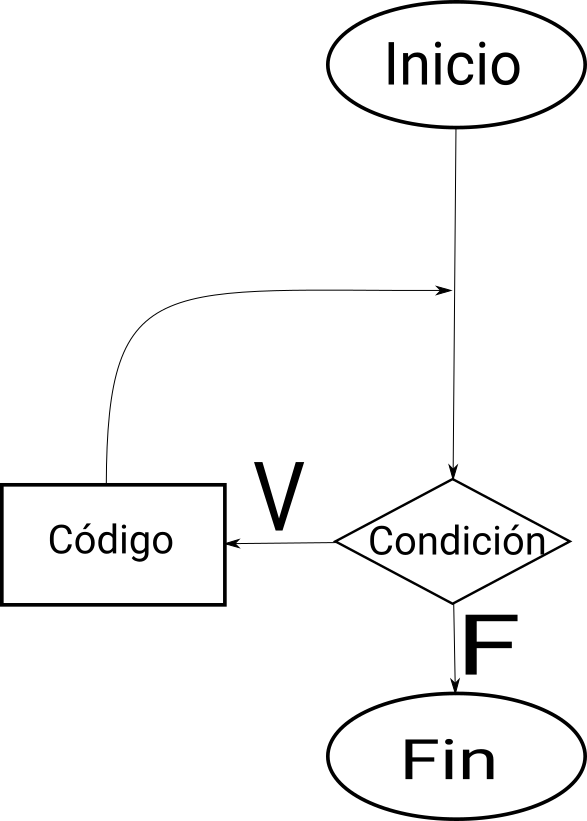
\includegraphics[width=.9\linewidth]{while.png}
\caption{Diagrama de un bucle while}
\end{figure}

Por ejemplo, si queremos un programa que muestre por pantalla los números del 1 al 10, podemos hacer lo siguiente:

\begin{verbatim}
class BucleWhile {

    public static void main(String[] args) {
	//Ponemos el número con el valor que queremos al principio
	int numeroActual=1;

	//Bucle while
	//Condición: que numeroActual sea menor o igual que 10
	while (numeroActual<=10) {

	    //Imprimimos por pantalla el número con su valor en este momento
	    System.out.println(numeroActual);

	    //Aumentamos el valor del número
	    //Si no lo hacemos, el valor de númeroActual siempre será menor o igual a 10 y tendremos un bucle infinito
	    numeroActual++;
	}
    }

}
\end{verbatim}
\captionof{figure}{\label{org6756d85}
Bucle While}
\subsection{El bucle for}
\label{sec:org8f21363}
El bucle \texttt{for} es un caso especial del bucle \texttt{while}, este bucle se va a ejecutar igualmente mientras se cumpla la condición dada, por lo que su diagrama es el mismo, pero nos permite simplificar la programación metiendo en la cabecera tanto la inicialización de la variable como su modificación, por ejemplo, si como en el caso anterior queremos escribir los números del 1 al 10 con un bucle \texttt{for} lo haríamos así:

\begin{verbatim}
class BucleFor {

    public static void main (String[] args) {
	for (int numeroActual=1; numeroActual<=10; numeroActual++) {
	    System.out.println(numeroActual);
	}
    }

}
\end{verbatim}
\captionof{figure}{\label{org4c70b2b}
Bucle For}

Como podemos ver, el resultado de este programa será exáctamente el mismo que el anterior:

La decisión de utiliar un tipo de bucle u otro depende del programador, pero se suele utiliar el bucle \texttt{for} para situaciones en las que haya que \emph{contar}, como en el caso que hemos puesto porque nos permite crear y deshechar la variable en la propia cabecera sin tener que llevar datos innecesarios, aunque por supuesto podemos usar una variable que tengamos de antes como en el bucle \texttt{while} e, incluso, no modificar la variable en la cabecera y hacerlo en el cuerpo.

\begin{verbatim}
class BucleForSinInicializacion {

    public static void main (String[] args) {
    int numeroActual=1;
    for (; numeroActual<=10; numeroActual++) {
	    System.out.println(numeroActual);
	}
    }

}
\end{verbatim}
\captionof{figure}{\label{org0834611}
Bucle For sin inicialización en la cabecera}

\begin{verbatim}
class BucleForSinModificacion {

    public static void main (String[] args) {
	for (int numeroActual=1; numeroActual<=10;) {
	    System.out.println(numeroActual);
	    numeroActual++;
	}
    }

}
\end{verbatim}
\captionof{figure}{\label{org0817b3f}
Bucle For Sin Modificacion en la cabecera}

Y, por supuesto, si sacamos de la cabecera tanto la inicialización como la modificación de la variable, lo que tenemos es un bucle \texttt{while} con otro nombre:

\begin{verbatim}
class BucleForSinInicializacionNiModificacion {

    public static void main (String[] args) {
	int numeroActual=1;
	for (; numeroActual<=10;) {
	    System.out.println(numeroActual);
	    numeroActual++;
	}
    }

}
\end{verbatim}
\captionof{figure}{\label{org2e7ff5e}
Bucle For Sin inicialización ni Modificacion en la cabecera}

\subsection{El bucle do-while}
\label{sec:org7f9bf19}
Hasta ahora hemos visto bucles que se ejecutan sólo si se cumple una determinada condición, pero ¿y si queremos que un fragmento de código se ejecute como mínimo una vez pero si se cumple la condición se ejecute unas cuantas mas? Podríamos duplicar el mismo código, una vez fuera del bucle y otra vez dentro, pero para ahorrarnos la reduncancia tenemos el bucle \texttt{do-while}.

Este bucle se trata de un bucle \texttt{while} en el que la condición para volverlo a ejecutar se encuentra al final y no al principio, fijémonos en el siguiente diagrama:

\begin{figure}[htbp]
\centering
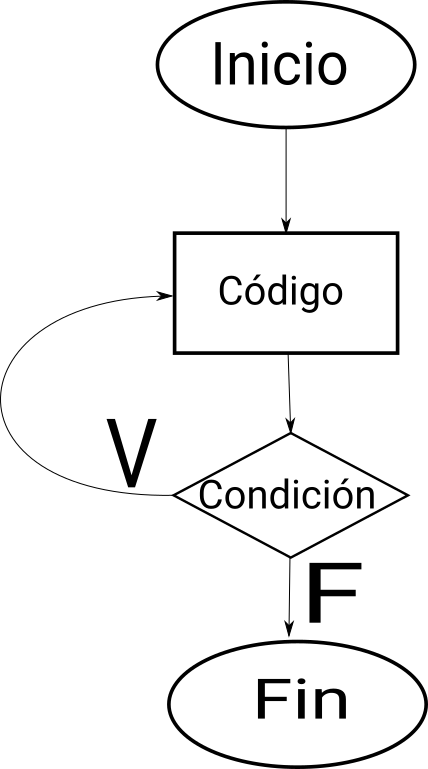
\includegraphics[width=.9\linewidth]{do-while.png}
\caption{Diagrama de un bucle do-while}
\end{figure}

Podemos continuar con nuestro ejemplo de contar de 1 a 10, veamos como se haría con un bucle do-while:

\begin{verbatim}
class DoWhile {

  public static void main(String[] args) {
    //Inicializamos la variable fuera del bucle
    int numeroActual=1;
    do {
      //Imprimimos su valor
      System.out.println(numeroActual);
      //Aumentamos la variable
      numeroActual++;
      //Comprobamos la condición, como ya se ejecuta una vez como mínimo
      //es necesario poner menor (<) y no menor o igual (<=), si lo hiciéramos
      //cuando el valor de numeroActual fuera 10 cumpliría y volvería a ejecutar
      //el código, por lo tanto contaría hasta 11
    } while (numeroActual < 10);
  }

}
\end{verbatim}
\captionof{figure}{\label{org96b6cf4}
Bucle do-while}

\section{Métodos y funciones}
\label{sec:orge0ce570}
Con lo que ya sabemos podemos crear programas muy potentes, podemos controlar si un bloque de código se ejecutará o no y cuantas veces lo hará, pero la ejecución sigue siendo \emph{de arriba a abajo}, estamos en lo que se conoce como \textbf{programación estructurada}, pero vayamos más allá, hasta ahora, si queríamos ejecutar un bloque de código más de una vez podíamos hacer bucles, pero estos siempre se ejecutarán con los mismos datos, con los métodos podemos ejecutar el mismo código pero con \textbf{parámetros} diferentes, veamos un ejemplo sencillo:

\begin{verbatim}
class MiPrimerMetodo {

  //Aquí tenemos el método main, no devuelve nada (void)
  //y recibe como parámetro un array de Strings (varias cadenas de texto)
  public static void main(String [] args) {
    //Creamos una variable llamada nombre y la inicializamos
    String nombre = "Bimo";
    //Llamamos a nuestro método y le pasamos como parámetro la variable
    saludar(nombre);
    //Cambiamos el valor de la variable
    nombre = "Kirby";
    //Y volvemos a llamar al método
    saludar(kirby);
  }

  //Aquí tenemos nuestro método, se llama saludar y no devuelve nada,
  //recibe como parámetro una cadena de texto llamada nombre,
  //cada vez que se ejecute saludará a quien venga escrito en la variable nombre
  static void saludar(String nombre) {
    System.out.println("Hola, "+nombre);
  }

}
\end{verbatim}
\captionof{figure}{\label{orge12e34c}
Mi primer método}

\section{Clases y objetos}
\label{sec:orgc770de8}
\end{document}